\documentclass[11pt,a4paper]{article}

\usepackage[margin=2.5cm]{geometry}
\usepackage{amsmath,amssymb}
\usepackage{hyperref}
\usepackage[T1]{fontenc}
\usepackage{tikz}
\usetikzlibrary{arrows.meta,positioning}

\title{Context Renormalization:\\
	A Bounded-Memory Protocol for Multi-Session LLM Work}

\author{
	Vasili Gavrilov \\
	\small Independent Researcher
	\and
	ChatGPT\,5.1 \\
	\small Large Language Model
}

\date{}

\begin{document}
	\maketitle
	
	\begin{abstract}
		Collaborations with Large Language Models (LLMs) often span multiple sessions. 
		Over time, these sessions produce design decisions, constraints, and other 
		knowledge that should be carried forward, yet most LLM interfaces impose finite 
		context windows, making naive accumulation infeasible. Furthermore, long 
		interactive exchanges frequently become slow or unstable, because the client 
		interface must maintain an increasingly large DOM tree and conversation 
		transcript. Users are therefore often forced to terminate the session and begin 
		a new one, at the cost of losing accumulated continuity.
		
		This paper introduces \emph{Context Renormalization}, a simple protocol for 
		maintaining a bounded-size `knowledge ledger'' summarizing essential results 
		of each session. At the end of each session, new information is appended as a 
		delta, and the ledger is compressed back to a fixed text size limit measured in 
		characters. A \emph{Compression Difficulty Score} (CDS) quantifies how hard 
		this compression is, signaling when knowledge should be externalized into 
		permanent documents or implemented in durable artifacts. The protocol is 
		vendor-agnostic: the ledger is plain text, interpretable by any LLM supporting 
		text rewriting. We illustrate the protocol with a two-session design exercise, 
		but the method applies broadly to any multi-session workflow.
	\end{abstract}
	
	\section{Overview}
	
	The protocol relies on a single text file, typically named \texttt{context.txt}, 
	stored with the main project artifacts. This file acts as a bounded, evolving 
	representation of the latent working memory accumulated across multiple LLM 
	interactions.
	
	In real usage, long-running interactions become slow due to large DOM trees, 
	long transcripts, and accumulated UI state. Users often restart the session to 
	regain responsiveness. Context Renormalization allows this safely: before 
	closing the sluggish session, the user requests a ledger update; the next 
	session then begins with the same distilled understanding provided by the ledger.
	
	At each end-of-session boundary, the user provides:
	\begin{itemize}
		\item the current \texttt{context.txt},
		\item any working materials (for example, code snapshots or notes),
		\item and the instruction:
	\end{itemize}
	
	\begin{quote}
		\emph{`End of session. Update context according to the control header protocol.''}
	\end{quote}
	
	The LLM then executes the renormalization algorithm.
	
	% ============================================================
	% SIMPLE, NON-TECHNICAL ILLUSTRATION FOR EARLY READERS
	% ============================================================
	
	\begin{figure}[h]
		\centering
		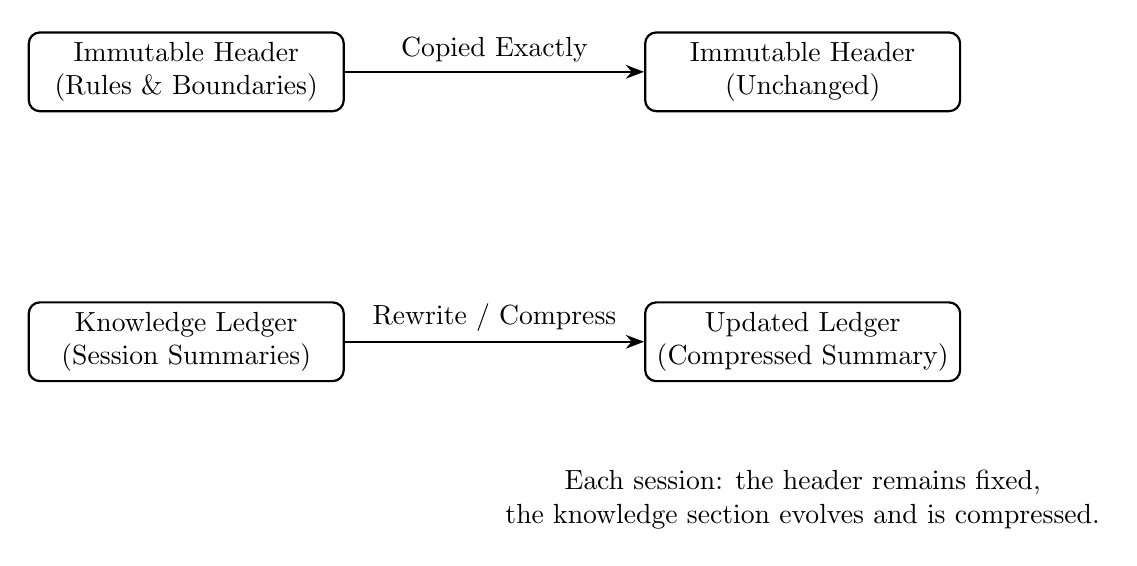
\begin{tikzpicture}[>=Stealth, node distance=2.4cm]
		
		\tikzstyle{box}=[draw, rounded corners, thick, minimum width=4cm,
		minimum height=1cm, align=center]
		
		% Initial header + ledger
		\node[box] (H1) {Immutable Header \\ (Rules \& Boundaries)};
		\node[box, below=of H1] (K1) {Knowledge Ledger \\ (Session Summaries)};
		
		% Next iteration
		\node[box, right=3.8cm of H1] (H2) {Immutable Header \\ (Unchanged)};
		\node[box, below=of H2] (K2) {Updated Ledger \\ (Compressed Summary)};
		
		% Arrows
		\draw[->, thick] (H1.east) -- node[above]{Copied Exactly} (H2.west);
		\draw[->, thick] (K1.east) -- node[above]{Rewrite / Compress} (K2.west);
		
		\node[below=1.0cm of K2, align=center]
		{Each session: the header remains fixed, \\ the knowledge section evolves and is compressed.};
		
		\end{tikzpicture}
		\caption{High-level illustration of Context Renormalization. The immutable header remains unchanged across sessions, while the knowledge ledger is rewritten and compressed to maintain bounded size.}
	\end{figure}
	
	% ============================================================
	
	\section{Structure of the Ledger}
	
	\subsection{Control Header}
	
	The control header appears at the top of \texttt{context.txt} and contains:
	\begin{itemize}
		\item \texttt{Session\_Count}: number of summarized sessions,
		\item \texttt{C\_max}: the fixed text size limit (in characters),
		\item the rules of the protocol,
		\item and edit boundaries:
		\begin{verbatim}
		=== BEGIN KNOWLEDGE REGION ===
		=== END KNOWLEDGE REGION ===
		\end{verbatim}
	\end{itemize}
	
	The header is immutable except for incrementing \texttt{Session\_Count}.
	
	\subsection{Knowledge Region}
	
	This is the editable, compressible portion of the file. It consists of 
	chronologically ordered summaries:
	
	\begin{verbatim}
	SESSION 1 --- Summary
	SESSION 2 --- Summary
	...
	SESSION N --- Summary
	\end{verbatim}
	
	Each summary contains durable insights: rules, decisions, invariants, structural 
	clarifications. Ephemeral reasoning is not preserved.
	
	\section{Renormalization Algorithm}
	\label{sec:algorithm}
	
	Let $C_{\max}$ denote the fixed text size limit (in characters). The algorithm proceeds:
	
	\begin{enumerate}
		\item Parse \texttt{context.txt} and increment \texttt{Session\_Count}.
		\item Append a new session summary containing only durable knowledge.
		\item Attempt to compress the knowledge region to remain within $C_{\max}$:
		\begin{itemize}
			\item merge redundant ideas,
			\item rewrite detailed episodes as general rules,
			\item compress older sessions more aggressively,
			\item remove content now encoded directly in project artifacts.
		\end{itemize}
		\item Compute the Compression Difficulty Score:
		\[
		CDS = \max(0, C_{\text{post,min}} - C_{\max}),
		\]
		where $C_{\text{post,min}}$ is the smallest character size achievable 
		without loss of intended meaning.
		\item If $CDS > 0$, include a warning for the user.
	\end{enumerate}
	
	This protocol is fully portable: any LLM capable of text rewriting can apply it.
	
	\section{Compression Difficulty Score}
	
	CDS quantifies representational pressure. It measures how far the final, 
	irreducible text size exceeds the allowed limit:
	
	\[
	CDS = \max(0, C_{\text{post,min}} - C_{\max}).
	\]
	
	Interpretation:
	\begin{itemize}
		\item $CDS = 0$: ledger compresses cleanly; no action needed.
		\item Small $CDS > 0$: mild pressure; consider externalizing knowledge.
		\item Large $CDS$: significant pressure; stabilize knowledge in more durable artifacts.
	\end{itemize}
	
	CDS relates conceptually to description length: it is a practical, operational 
	estimate of the textual complexity of the knowledge state.
	
	\section{Boundedness and Project Phases}
	
	As the session count grows, the ledger must represent more history within the 
	same character limit. Older sessions are compressed into concise statements, 
	but never removed entirely.
	
	At natural project milestones, the ledger can be externalized into permanent 
	documents, and a new ledger can begin with \texttt{Session\_Count = 1}. Thus, 
	the ledger functions primarily as a bounded working memory for an active 
	phase of development, while its compressed snapshots may also serve as a 
	lightweight historical record useful for later analysis, knowledge transfer, 
	or organizational learning.
	
	\section{Cross-Model and Cross-Vendor Use}
	
	The protocol:
	\begin{itemize}
		\item uses plain text only,
		\item does not depend on model-specific memory,
		\item defines its own update rules explicitly in the header.
	\end{itemize}
	
	Therefore, any LLM---regardless of provider or version---can update 
	\texttt{context.txt} as long as it follows the rules. The ledger becomes a 
	portable, model-agnostic mechanism for continuity.
	
	\section{Two-Session Example}
	
	A real design exercise produced a substantial amount of raw dialogue and code. 
	After renormalization with $C_{\max}$ set appropriately, the ledger captured:
	\begin{itemize}
		\item architectural invariants,
		\item structural relationships and rules,
		\item concise summaries of each session,
		\item and no redundant reasoning fragments.
	\end{itemize}
	
	CDS for the first sessions was zero, demonstrating effective compression under 
	the chosen limit.
	
	\section{Related Work and Positioning}
	
	Context Renormalization intersects with several known areas yet differs in 
	important ways.
	
	\subsection*{Conversational Memory and Recursive Summarization}
	
	Work on long-term conversational memory uses recursive or hierarchical 
	summarization to maintain continuity across long interactions. These techniques 
	typically optimize for model performance under finite context windows, whereas 
	Context Renormalization defines a portable, explicit, user-facing ledger with 
	session semantics and a character limit.
	
	\subsection*{Long-Document Summarization and Multi-Stage Compression}
	
	Multi-stage summarization compresses long documents using repeated 
	summarization. Context Renormalization applies a similar idea, but to an 
	evolving project-level knowledge file rather than a static text, and with an 
	explicit rule that older sessions are compressed more aggressively while each 
	session remains represented.
	
	\subsection*{External Memory Systems and Retrieval-Augmented Models}
	
	External memory systems store persistent knowledge in retrievable formats. 
	By contrast, Context Renormalization uses a minimal plain-text ledger requiring 
	no infrastructure, indexing, or retrieval; its portability arises from its 
	simplicity and explicit protocol.
	
	\subsection*{Information Compression and Description Length}
	
	The protocol is conceptually related to minimum description length: the ledger 
	is a bounded textual representation of project knowledge. CDS provides an 
	operational estimate of representational pressure. True Kolmogorov complexity 
	is uncomputable, but the protocol implements a practical, observable 
	approximation by asking the LLM to compress as much as possible without losing 
	essential meaning.
	
	\subsection*{Positioning}
	
	Context Renormalization is not a new summarization algorithm; it is a protocol 
	that combines:
	\begin{itemize}
		\item a fixed-size ledger,
		\item explicit update rules,
		\item fairness across sessions,
		\item and a quantitative compression signal.
	\end{itemize}
	
	It provides a simple, portable method for maintaining continuity across LLM 
	sessions.
	
	\section{Discussion}
	
	The protocol assumes the LLM can identify redundancy and summarize 
	appropriately. Different models may produce different compression patterns, 
	but the constraints remain stable. Chronic CDS pressure indicates the need to 
	externalize or implement knowledge to maintain boundedness.
	
	Beyond its immediate engineering role, a sequence of compressed ledgers can 
	also be viewed as a historical trace of a particular human--LLM collaboration. 
	Each renormalized context encodes not only technical decisions, but also the 
	approaches, practices, and stylistic patterns that shaped those decisions at 
	a given time. If a project later proves successful relative to comparable 
	efforts, these snapshots may themselves become research artifacts: a compact 
	record of how knowledge, conventions, and design heuristics evolved under 
	bounded-memory constraints.
	
	\subsection*{Organizational Applications}
	
	In organizational settings, a sequence of renormalized contexts can serve as a 
	valuable form of knowledge capture. Each compressed ledger provides a distilled 
	trace of how a particular practitioner interacts with an LLM: their methods, 
	heuristics, strategies of decomposition, and patterns of inquiry. Over time, 
	these traces form a compact representation of an individual's style of work.
	
	Such records may reveal differences in method among collaborators that correlate 
	with effectiveness or creativity. Organizations may analyze these traces to 
	identify best practices, extract transferable techniques, and elevate them into 
	shared standards or onboarding material. In this sense, the ledger supports 
	organizational learning by converting tacit knowledge into explicit form.
	
	Moreover, these preserved traces may surface forms of innovation that would 
	otherwise remain hidden inside unlogged or ephemeral interactions. Many 
	innovative strategies arise not from formal processes but from spontaneous 
	tactics used during day-to-day problem solving. By compressing and preserving 
	these interactions in a structured and comparable form, the ledger makes such 
	tacit experimentation visible. This visibility enables organizations to detect 
	emerging techniques, understand how they differ from conventional practice, 
	and potentially convert them into formalized innovations, training material, or 
	new internal standards.
	
	% ============================================================
	% FUTURE WORK --- METALANGUAGE (TEXT PLUS FORMAL VIEW)
	% ============================================================
	
	\section*{Future Work: A Metalanguage for Recursive LLM Coordination}
	
	Context Renormalization suggests the need for a formal \emph{metalanguage} for
	LLM-to-LLM continuity. The protocol already separates an immutable header---defining
	rules, constraints, and boundaries---from a mutable region that each LLM
	rewrites under bounded compression. This division acts as a meta-level contract:
	the header encodes operational semantics; the ledger encodes evolving state.
	
	Each session constitutes a recursive step: a new LLM receives the immutable
	instructions, transforms the mutable region, and emits a successor ledger. A
	natural research direction is to formalize this process by defining:
	\begin{enumerate}
		\item a typed grammar for the header-language,
		\item machine-checkable invariants for summaries,
		\item forward-compatible rules enabling heterogeneous models to participate,
		\item optional verification that each renormalization obeys the contract.
	\end{enumerate}
	
	Such a metalanguage would make Context Renormalization a general inter-LLM
	coordination mechanism---governing not only what is preserved, but how compression
	and rewriting are interpreted across recursive iterations---thus enabling stable,
	portable continuity across models and vendors.
	
	\bigskip
	
	Formally, each renormalization step can be viewed as the application of an
	operator:
	\[
	S_{n+1} = R_H(S_n),
	\]
	where $H$ is the immutable header defining the rules of the protocol, and
	$S_n$ is the knowledge ledger state after $n$ sessions. The operator $R_H$ is
	fully determined by $H$, and its repeated application defines the recursive
	flow illustrated below.
	
	\bigskip
	
	\begin{figure}[h]
		\centering
		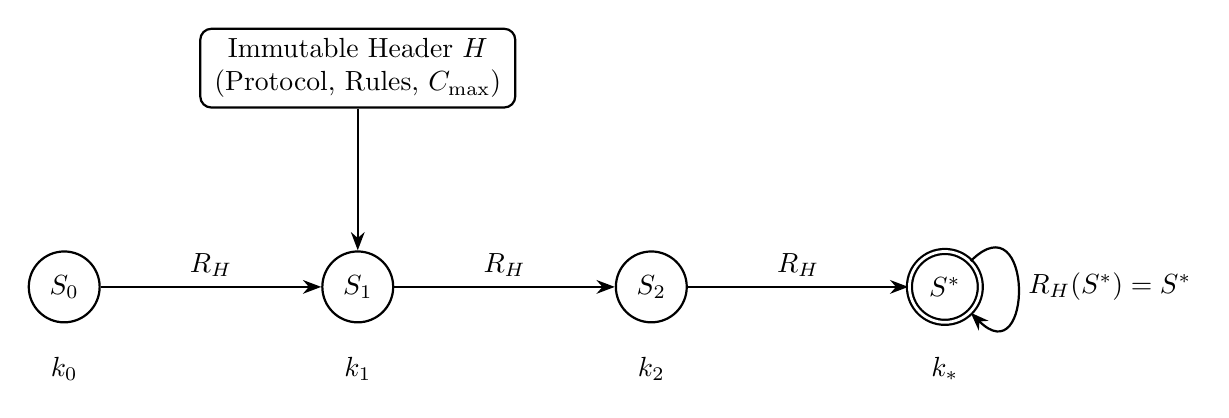
\begin{tikzpicture}[>=Stealth, node distance=2.8cm]
		
		\tikzstyle{state}=[circle, draw, thick, minimum size=0.9cm, align=center]
		\tikzstyle{fpstate}=[circle, double, double distance=1pt, draw, thick,
		minimum size=0.9cm, align=center]
		\tikzstyle{header}=[draw, rounded corners, thick, align=center,
		minimum width=4cm, minimum height=1cm]
		
		% States S_0, S_1, S_2, S*
		\node[state] (s0) {$S_0$};
		\node[state, right=of s0] (s1) {$S_1$};
		\node[state, right=of s1] (s2) {$S_2$};
		\node[fpstate, right=of s2] (sf) {$S^\ast$};
		
		% Scale labels
		\node[below=0.3cm of s0] {$k_0$};
		\node[below=0.3cm of s1] {$k_1$};
		\node[below=0.3cm of s2] {$k_2$};
		\node[below=0.3cm of sf] {$k_\ast$};
		
		% Flow arrows
		\draw[->, thick] (s0) -- node[above] {$R_H$} (s1);
		\draw[->, thick] (s1) -- node[above] {$R_H$} (s2);
		\draw[->, thick] (s2) -- node[above] {$R_H$} (sf);
		
		% Fixed-point loop
		\draw[->, thick] (sf.north east) .. controls +(0.8,0.8)
		and +(0.8,-0.8)
		.. node[right] {$R_H(S^\ast)=S^\ast$}
		(sf.south east);
		
		% Header H
		\node[header, above=1.8cm of s1] (Hnode)
		{Immutable Header $H$ \\ (Protocol, Rules, $C_{\max}$)};
		
		% Influence arrow
		\draw[->, thick] (Hnode.south) .. controls +(0,-0.7) .. (s1.north);
		
		\end{tikzpicture}
		\caption{Renormalization-group view of Context Renormalization. The immutable
			header $H$ defines the operator $R_H$, which maps each compressed ledger
			$S_n$ to its successor $S_{n+1}$. The flow may approach a fixed point
			$S^\ast$ satisfying $R_H(S^\ast)=S^\ast$, representing a stable encoding
			of the project under bounded-memory constraints.}
	\end{figure}
	
	\section{Conclusion}
	
	Context Renormalization supports continuity across multiple LLM interactions 
	under strict size constraints. By combining explicit rules, bounded 
	representations, and a compression difficulty signal, it enables safe session 
	restarts, portability across models, and efficient collaboration.
	
	\appendix
	
	\section{Full Example Ledger (context.txt)}
	Real project ledger produced by two LLM sessions with a software developer.
	
	\begin{verbatim}
	============================================================
	CONTEXT PROTOCOL (DO NOT EDIT OR COMPRESS)
	============================================================
	Version: 1
	Context_Session_Count: 2        # Increase by 1 for each major "day session"
	Context_Total_Budget_Characters: 20000   # Target compressed size in characters
	
	Purpose:
	- This file is a long-lived, machine-readable knowledge-transfer document.
	- It encodes project-specific conventions, invariants, and design intent.
	- The actual codebase (SQL/Java/Servlets/Tests/React) remains the primary
	source of truth; this file explains "how to read and extend it".
	
	Compression / Fairness Principle:
	- Let N = Context_Session_Count (number of major sessions summarized).
	- After compression, this file should be approximately 
	Context_Total_Budget_Characters characters.
	- Each session's knowledge should have comparable informational weight
	(roughly 1/N of the file, up to judgment).
	- As N grows, older sessions are summarized more aggressively, but never
	entirely erased.
	
	Update Protocol (for future ChatGPT sessions):
	1) When the user uploads this context.txt + code and clearly indicates
	"END OF DAY / UPDATE CONTEXT ACCORDING TO CONTEXT PROTOCOL":
	- Read context.txt fully and inspect the current code.
	- Increment Context_Session_Count by 1 in the CONTEXT PROTOCOL header only.
	2) Append a new "SESSION <N> --- KNOWLEDGE SUMMARY" block at the *end* of the
	KNOWLEDGE REGION summarizing what is NEW/CHANGED today:
	- New conventions, schema changes, endpoint behavior, invariants.
	- Do NOT restate what is obviously encoded in the current code or
	already clearly described in previous session blocks.
	3) If total character length > Context_Total_Budget_Characters:
	- Compress older session sections:
	• Merge duplicates.
	• Remove verbose narrative.
	• Replace long examples with rules or references to code/REST docs.
	- Prefer compressing content that is now clearly represented in the
	codebase (schema, servlet endpoints, tests).
	- Every session must retain at least a concise summary of:
	• What was done that session.
	• What rules/invariants it introduced or changed.
	4) DO NOT:
	- Modify or delete this CONTEXT PROTOCOL block.
	- Compress lines outside the KNOWLEDGE REGION markers.
	
	Knowledge Region Markers:
	- Only lines between the following markers may be edited/compressed:
	- "=== BEGIN KNOWLEDGE REGION ==="
	- "=== END KNOWLEDGE REGION ==="
	@author Vasili Gavrilov 09/12/2025
	
	============================================================
	=== BEGIN KNOWLEDGE REGION =================================
	============================================================
	
	============================================================
	SESSION 1 --- GLOBAL BACKEND, STYLE, REST, DAO, TESTS
	(Original "Become the Same Assistant" Context)
	============================================================
	
	[1. Global Development Philosophy]
	Goal: minimal entropy; SQL as source of truth.
	No ORMs, no heavy frameworks, no complex routing.
	Java is thin glue:
	DAO = "SQL + JSON builder"
	Servlet = "path parsing + auth + call DAO + send JSON"
	No domain POJOs except USER (for login/validation).
	All server responses are JSON; errors are JSON objects with an "error" field.
	
	[2. Core Architectural Pattern]
	Single main servlet: RestServlet.
	URL path parsing:
	request.getPathInfo() -> split into segments.
	Switch on path.get(0) (top-level resource).
	Branch on path length (n) and specific suffix segments.
	Examples:
	GET /models -> list models.
	GET /models/{id}/runs -> runs for model.
	Each endpoint block is clearly separated by comment banner.
	
	[3. REST Endpoint Design Rules]
	Each endpoint documented in RESTapi.txt using:
	<Object> -- <Action>
	Path:
	Client:
	Server:
	Errors:
	Notes:
	RESTapi-examples.txt mirrors titles but contains only curl examples.
	New endpoints require six steps:
	1) Write SQL.
	2) Add DAO method.
	3) Add servlet handler.
	4) Add tests.
	5) Update RESTapi.txt.
	6) Update RESTapi-examples.txt.
	No endpoint is done until all six steps are complete.
	
	[4. JSON & Naming Conventions]
	JSON fields use lowercase snake_case.
	Single object -> JSONObject; lists -> JSONArray.
	Errors always JSON {"error":"message"}.
	
	[5. SQL Style & DAO Pattern]
	SQL is primary design artifact; create.sql defines schema.
	Each DAO method:
	Begins with commented SQL block for debugging.
	Uses one-clause-per-line Java query string.
	Uses ConnectionProvider.getConnection().
	Closes ResultSet, PreparedStatement, Connection in finally.
	Returns JSON (never null).
	Avoid redundant checks when SQL enforces correctness.
	Prefer one expressive query over several small ones.
	
	[6. Authentication Rules]
	Public endpoints:
	status, login, register, users/send_registration,
	password_reset/*, static assets.
	All others require auth token:
	Header Authorization: Bearer <token>.
	GET fallback ?token=...
	Tokens in VALID_TOKEN.
	Error codes:
	missing_authentication_token,
	invalid_or_expired_token,
	user_not_found.
	
	[7. Testing Conventions]
	Every endpoint has regression test.
	Tests must be DB-idempotent.
	Flow:
	Login to get token.
	Call endpoint.
	Check HTTP status.
	Check JSON.
	Cleanup DB rows.
	Use TestUtil helpers.
	Error tests check status and message.
	Success tests check fields.
	
	[8. Core Schema (High-Level)]
	USER: email, password_hash, timestamps, registration token.
	ROLE, USER_ROLE: roles ADMIN, USER, STUDY_ADMIN.
	VALID_TOKEN: active login tokens.
	MODEL_PROVIDER: catalog of model providers.
	MODEL: model_name unique.
	EVAL_SET: asset sets.
	RUN: model execution using eval sets.
	ASSET: uri + mime, unique uri.
	ASSET_SET: eval_set_id <-> asset_id.
	STUDY_TEMPLATE: reusable templates.
	STUDY: experiment; links to RUN via STUDY_RUN.
	SCORE_CARD: aggregated metrics.
	STUDY_TASK_RUN_SCORE: per-task per-run metrics.
	
	[9. Performance Principles]
	Study design is low-volume; slower OK.
	Study execution is high-volume; must be optimized.
	Avoid redundant SELECTs.
	Prefer joins over multiple queries.
	Return empty arrays over 404 when ID optional.
	Use indexes to support filters.
	
	============================================================
	SESSION 2 --- STUDY / PAGE / QUESTION / ANSWER / ASSET SCHEMA
	(Annotation Layer and Page Types)
	============================================================
	
	[1. Conceptual Annotation Model]
	Goal: configurable study pages where annotators see assets and answer questions.
	Key entities:
	STUDY: experiment config.
	PAGE: one screen.
	PAGE_TYPE: layout semantics.
	ASSET: content item.
	ASSET_ON_PAGE: assets on page.
	QUESTION: prompts.
	ANSWER: responses.
	ANSWER_ASSET: per-asset overlays.
	STUDY_TASK: one participant session.
	RUN: model execution.
	
	[2. The Four Canonical Page Types]
	
	Type 1 --- One Asset, Many Questions
	One asset on page.
	Multiple questions about that asset.
	ANSWER_ASSET optional because asset is implied by PAGE.
	
	Type 2 --- Many Assets, One Shared Question
	Many assets.
	One question applies to all.
	ANSWER_ASSET includes one row per asset.
	
	Type 3A --- Many Assets, Multi-Select (Checkbox)
	Many assets.
	User selects any subset.
	chosen=1 for selected, 0 or absent otherwise.
	
	Type 3B --- Many Assets, Single-Select (Radio)
	Same as 3A but exactly one chosen=1.
	
	Type 4 --- Many Assets, One Question per Asset
	Each asset has corresponding question.
	Mapping implicit via ordering or explicit via QUESTION_ASSET.
	
	[3. Design-Time Schema Layer]
	PAGE: PK (study_id, page_num).
	ASSET_ON_PAGE: PK (study_id, page_num, asset_id).
	QUESTION: PK question_id; FK (study_id, page_num).
	display_order avoids duplicates.
	QUESTION_ASSET optional many-to-many.
	
	[4. Runtime Schema Layer]
	STUDY_TASK: represents user session.
	ANSWER: per-question; holds text/number payloads.
	ANSWER_ASSET: per-asset flags/scores/text.
	
	[5. Cardinalities and Invariants]
	STUDY -> PAGE.
	PAGE -> QUESTION.
	PAGE -> ASSET_ON_PAGE.
	QUESTION -> ANSWER.
	ANSWER <-> ASSET via ANSWER_ASSET.
	Type-specific invariants:
	Type1: one asset.
	Type2/3: multiple assets, one question.
	Type3B: exactly one chosen.
	Type4: questions equal assets.
	A possible extension: saving the fully compressed knowledge as compact history.
	
	[6. Minimal-Entropy Rules]
	ANSWER holds only question-level data.
	ANSWER_ASSET holds per-asset flags and values.
	QUESTION_ASSET optional.
	PAGE_TYPE encodes behavioral semantics.
	Compression reduces narrative when code expresses behavior.
	
	[7. API Behavior]
	Endpoints expose PAGE with:
	page_type,
	assets,
	questions,
	answers (with per-asset overlays).
	Write endpoints accept array of answers.
	Errors follow global conventions.
	
	============================================================
	=== END KNOWLEDGE REGION ===================================
	============================================================
	\end{verbatim}
	
\end{document}